%\usepackage{listings}
%\usepackage{xcolor}
\renewcommand\lstlistingname{Source Code}
\renewcommand\lstlistlistingname{Source Code}

% Define a custom style
\lstdefinestyle{myStyle}{
	backgroundcolor=\color{backcolour},   
	commentstyle=\color{codegreen},
	keywordstyle=\color{codeorange},
	numberstyle=\tiny\color{codegray},
	stringstyle=\color{codegreen},
	basicstyle=\ttfamily\footnotesize,
	breakatwhitespace=false,         
	breaklines=true,
	captionpos=b,                 
	keepspaces=true,                 
	numbers=left,       
	numbersep=5pt,                  
	showspaces=false,                
	showstringspaces=false,
	showtabs=false,                  
	tabsize=2,
	xleftmargin=10pt,
}


%-------------------------------------------------------------------
\chapter{Results}
\label{c:results}
%-------------------------------------------------------------------
The results section presents the outcomes of the modeling and methodology applied in this project, focusing on the performance of the machine learning model, insights gained from the dataset, and an evaluation of the overall quality of the system. These results demonstrate the effectiveness of the approach and provide a basis for assessing the project's success in achieving its objectives.

The trained Convolutional Neural Networks (CNNs) were evaluated on the test dataset to measure its ability to accurately recognize patterns in cardboards. Different models were used which include DenseNet, ResNet, VGG and MobileNet. For classification task, it was very important for the object to be correctly recognized in any given scenario. The results highlight how the choice of technique for image recognition and object detection significantly impacts model performance, as shown below.

%-------------------------------------------------------------------
\section{Object Detection without Annotations:}
%-------------------------------------------------------------------
In case of object detection without annotations, it can be seen that the area of focus where object can be found is quite large and the predictions sometimes are wrong. In case of images with very tiny details, this can cause errors.

\begin{figure}[H]
	\centering
	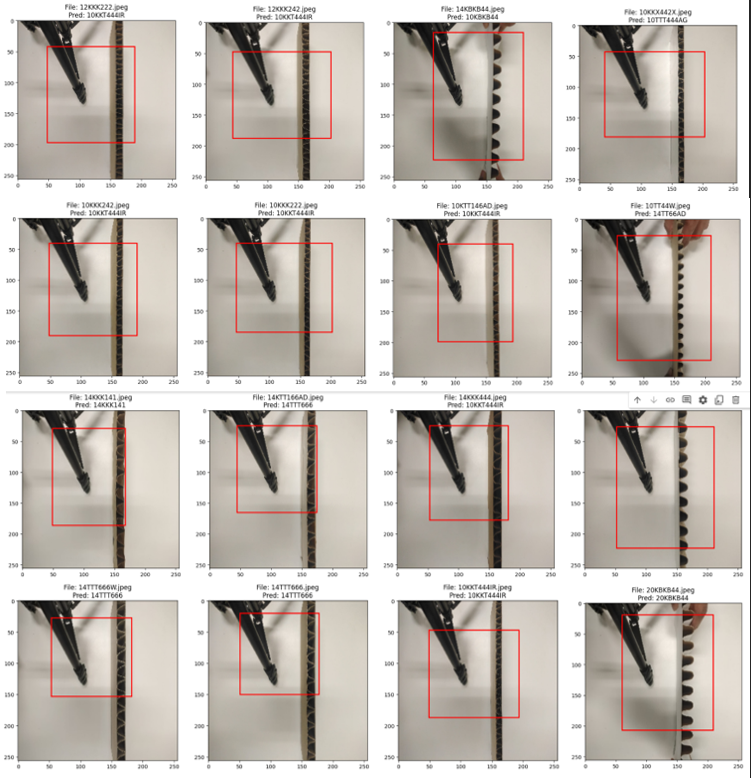
\includegraphics[width=0.6\textwidth]{figs/OBA51}
	\captionof{figure}{Object Detection without Annotations}
	\label{fig:OBA51}
\end{figure}

%-------------------------------------------------------------------
\section{Use of Annotations for Training Dataset:}
%-------------------------------------------------------------------
So, to improve object detection, the images were trained on annotated data, to detect the object with better accuracy.

\begin{figure}[H]
	\centering
	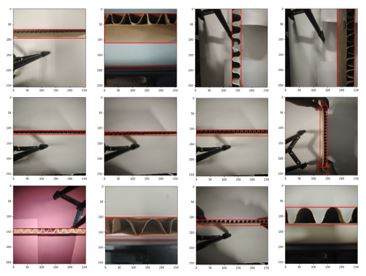
\includegraphics[width=0.6\textwidth]{figs/TD}
	\captionof{figure}{Use of Annotations for Training Dataset}
	\label{fig:TD}
\end{figure}
%-------------------------------------------------------------------
\section{Object Detection on Test Images After Annotations:}
%-------------------------------------------------------------------
After training on annotated images, it can be seen that the bounding boxes for object detection are detecting object in quite a better way. It's still not at peak accuracy as would be required for very detail oriented and specific data and to achieve that goal, instance segmentation has been applied, which is discussed later.

\begin{figure}[H]
	\centering
	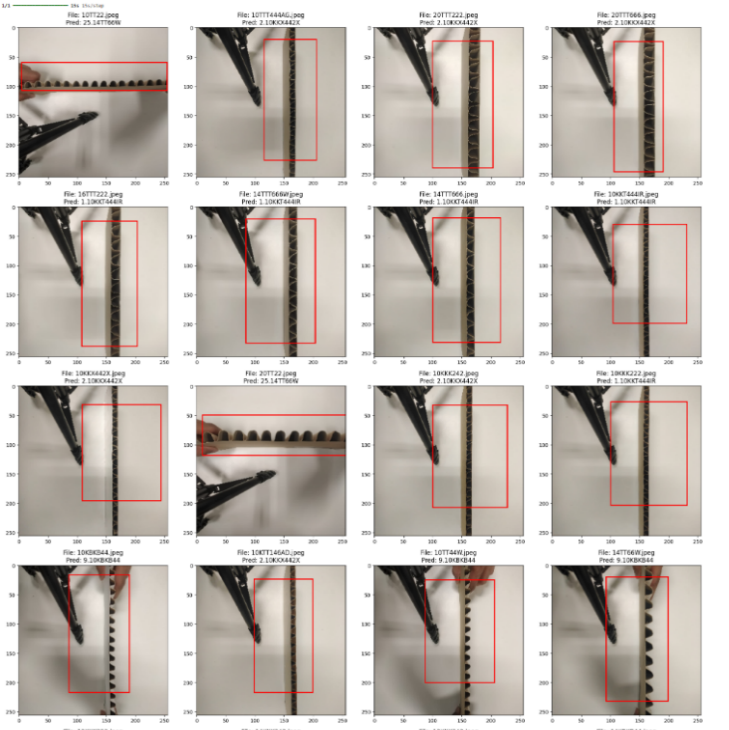
\includegraphics[width=0.5\textwidth]{figs/AA}
	\captionof{figure}{Object Detection on Test Images After Annotations}
	\label{fig:AA}
\end{figure}

%-------------------------------------------------------------------
\section{Impact of Data Augmentation:}
%-------------------------------------------------------------------

Data augmentations were removed, because they negatively impacted the model's performance. As the patterns closely resemble each other, augmentations made it difficult for model to classify after augmentations were applied. 

\begin{figure}[H]
	\centering
	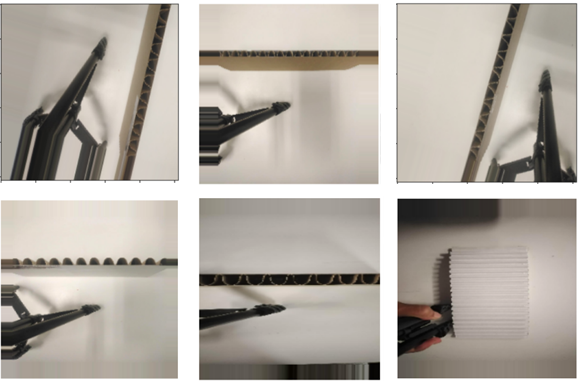
\includegraphics[width=0.5\textwidth]{figs/DA}
	\captionof{figure}{Impact of Data Augmentation}
	\label{fig:DA}
\end{figure}


As can be seen in the figure above, some images are stretched, changing the length, some of them are contracted and others are distorted from sides. This creates a dataset which is not good for training in cases where distance between two consecutive patterns, their length and all the other measurements matter.

Therefore, only augmentation techniques, such as rotations and flips were applied to enhance the dataset's diversity. These augmentations proved effective in improving the model's robustness to variations in the input images, as evidenced by the model's high accuracy and generalization capabilities.


%-------------------------------------------------------------------
\section{Results after Instance Segmentation:}
%------------------------------------------------------------

The integration of YOLOv8 with other machine learning models further enhances the model's capabilities for pattern recognition tasks involving complex objects. Collaborating with ensemble approaches or incorporating additional deep learning architectures yield synergistic effects that improve overall recognition performance. This multifaceted approach acknowledged the unique characteristics of cardboard flutes, allowing for finer distinctions based on complex shape variants and intricate designs.
The instance segmentation results showed good accuracy. It was able to detect accurately the mask of the testing images on which it was not trained and the accuracy was really good considering that it was trained on only few images.

\begin{figure}[H]
	\centering
	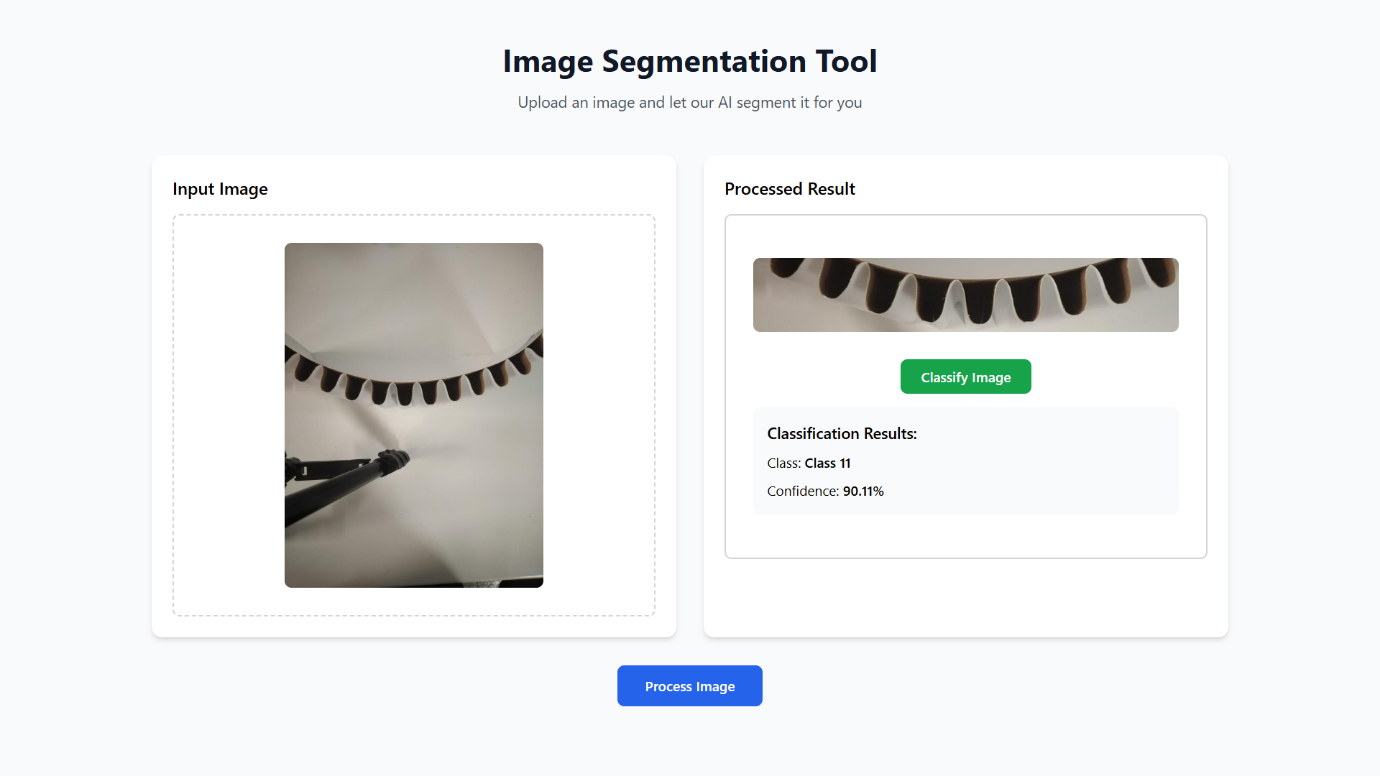
\includegraphics[width=0.9\textwidth]{figs/IST}
	\captionof{figure}{Folded Carton}
	\label{fig:IST}
\end{figure}


It can be seen in the picture above that it is able to detect the mask even in the case of folded carton.
Also, the object can be placed at any place in the image.

\begin{figure}[H]
	\centering
	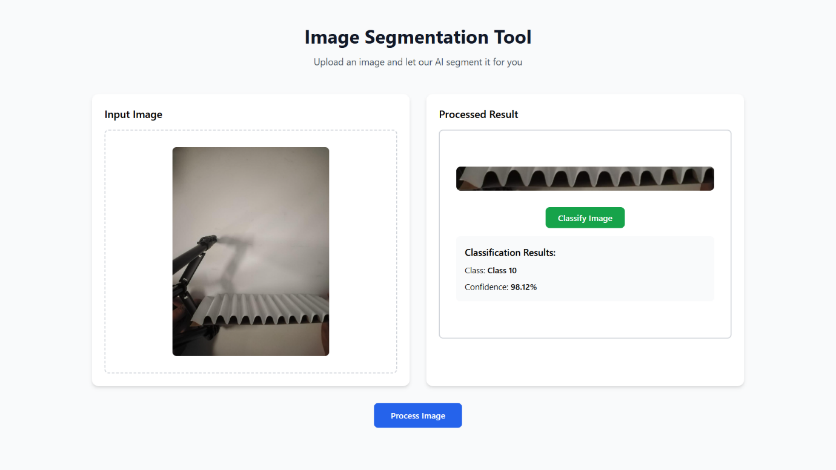
\includegraphics[width=0.9\textwidth]{figs/IST2}
	\captionof{figure}{Accurate Image Detection, when the object is at bottom}
	\label{fig:IST2}
\end{figure}

\begin{figure}[H]
	\centering
	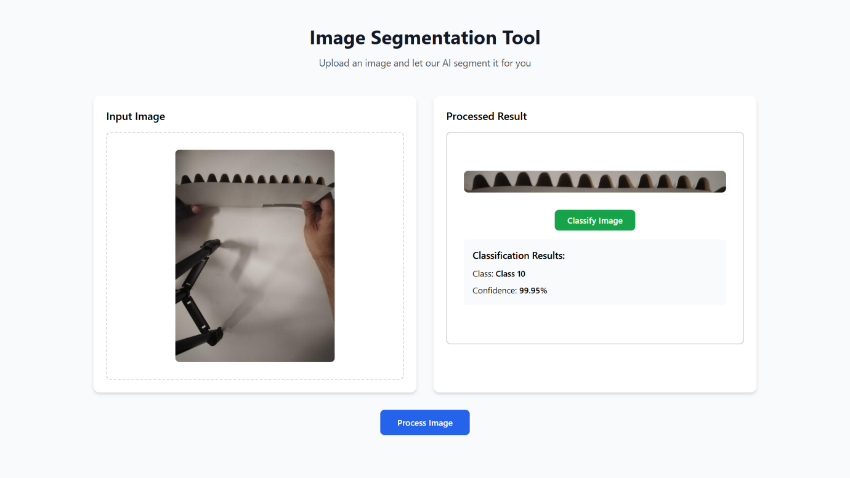
\includegraphics[width=0.9\textwidth]{figs/IST3}
	\captionof{figure}{Accurate Image Detection, when the object is at top.}
	\label{fig:IST3}
\end{figure}


For untrained images, the combined approach showed varied results for classification as can be seen in the picture below. The detection in this image is correct, but the confidence score is moderately low.

\begin{figure}[H]
	\centering
	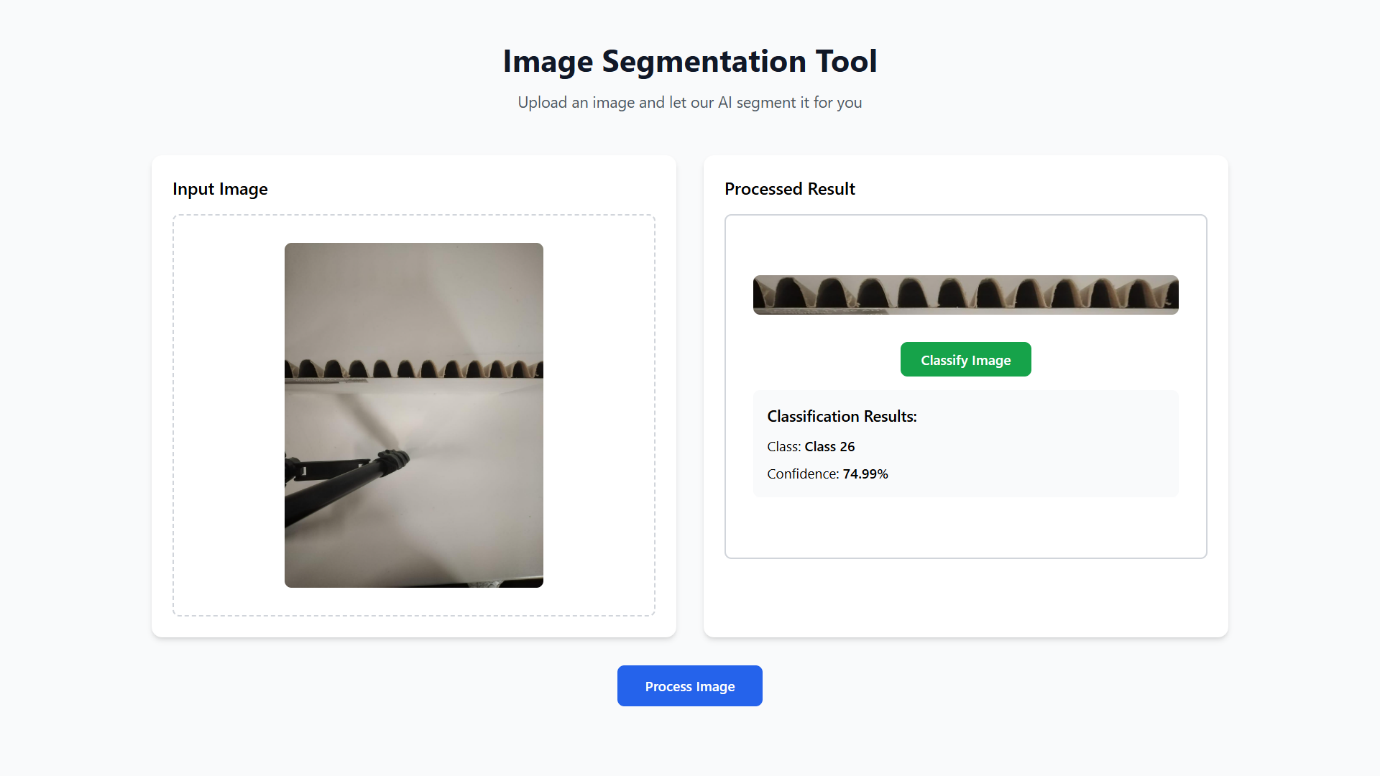
\includegraphics[width=0.9\textwidth]{figs/IST4}
	\captionof{figure}{Image Classification on Untrained Image}
	\label{fig:IST4}
\end{figure}

However, it is notable that for images taken from close distance, the model showed better accuracy as there were more images from close distance.

\begin{figure}[H]
	\centering
	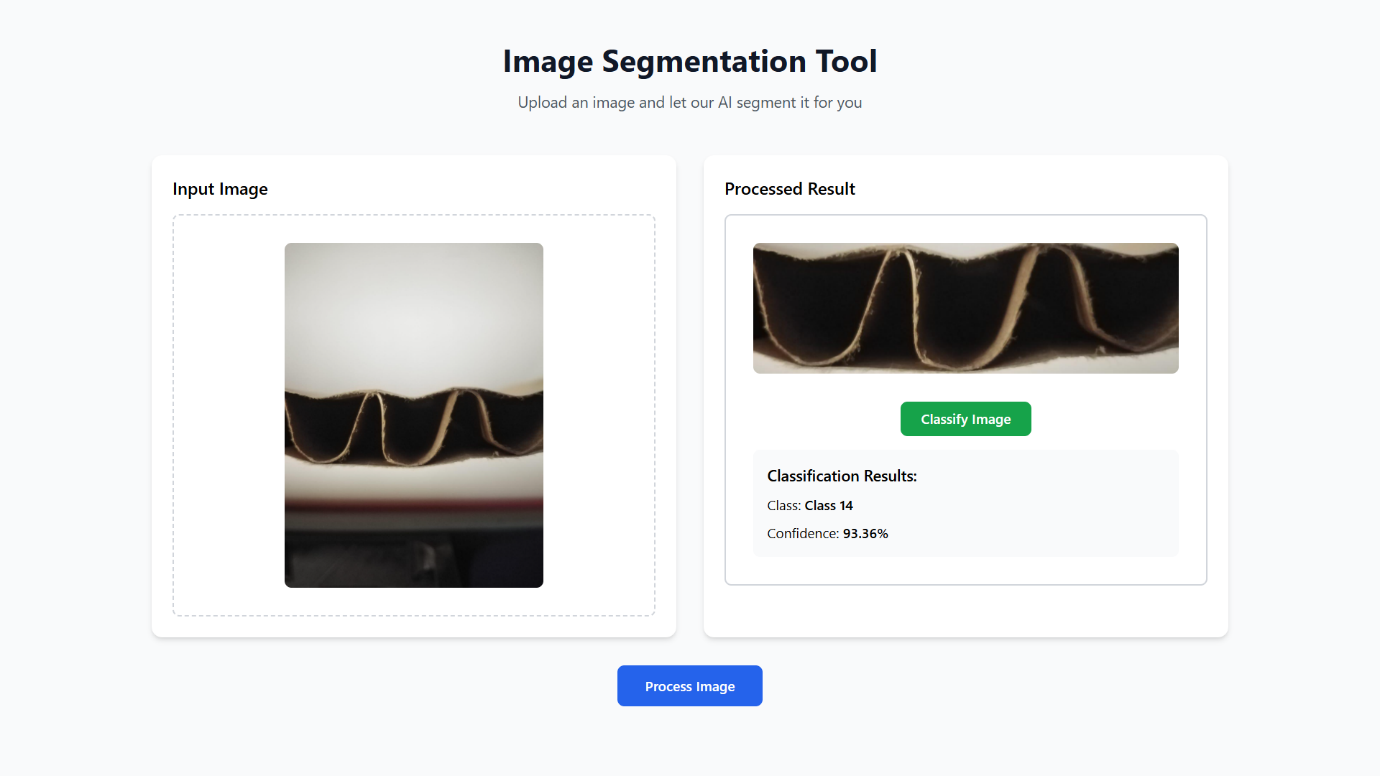
\includegraphics[width=0.8\textwidth]{figs/IST5}
	\captionof{figure}{Close Distance Image}
	\label{fig:IST5}
\end{figure}



%--------------------------------------------------------------------------
\section{Result on Trained Dataset}
%-------------------------------------------------------------------

Training images were also passed through the model to see if the accuracy plotted during training process equates to the actual accuracy. The trained data results were highly motivating, as the model accurately predicted them each time. On trained images, the confidence score varied between 99-100 percent and all the detections were accurate, underlining the successful training process.


%--------------------------------------------------------------------------
\section{System Reliability:}
%-------------------------------------------------------------------
The system's reliability was tested under various conditions, including changes in lighting, background, and image quality. The model consistently performed well, indicating that the system is robust and capable of handling the variability encountered in real-world environments, provided that image dataset is increased, as can be seen with the close distance images.

As can be seen in the image below, there is a hand that is covering some part of the actual image, still the model is able to detect with the remaining available part that there is a cardboard flute in the image and it belongs to this category. So, with these results it can be correctly said that the model is able to detect mask accurately and also classify the images correctly in case of pictures taken from close distance.

\begin{figure}[H]
	\centering
	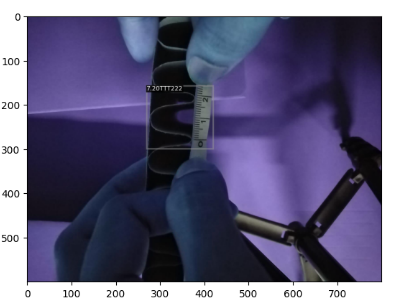
\includegraphics[width=0.6\textwidth]{figs/SR}
	\captionof{figure}{Accurate Mask detection, even in case of noise}
	\label{fig:SR}
\end{figure}


%--------------------------------------------------------------------------
\section{Scalability}
%-------------------------------------------------------------------
The system was designed with scalability in mind, allowing it to be easily adapted to different production lines, cardboard types, and inspection scenarios. The modular architecture and flexible deployment options (edge or cloud) ensure that the system can scale to meet the needs of different industrial applications.






%--------------------------------------------------------------------------
\section{Analysis of Training Results}
%-------------------------------------------------------------------
This section evaluates the effectiveness of machine learning models in classifying cardboard flutes based on the training outcomes recorded during the model training phase. It focuses on performance metrics, validation results, and the impact of training methodologies on classification accuracy. A comparative analysis of various deep learning architectures employed in this study reveals differences in accuracy rates, indicating that selection of the model can significantly affect the overall outcome. 

The comparative accuracy rates among the different architectures utilized showed that models such as DenseNet consistently outperformed others, achieving higher classification accuracy. But these comparisons, highlight the flexibility and context of application that these models possess, each catering to specific strengths in recognizing intricate patterns typical of cardboard flutes.

\begin{figure}[H]
	\centering
	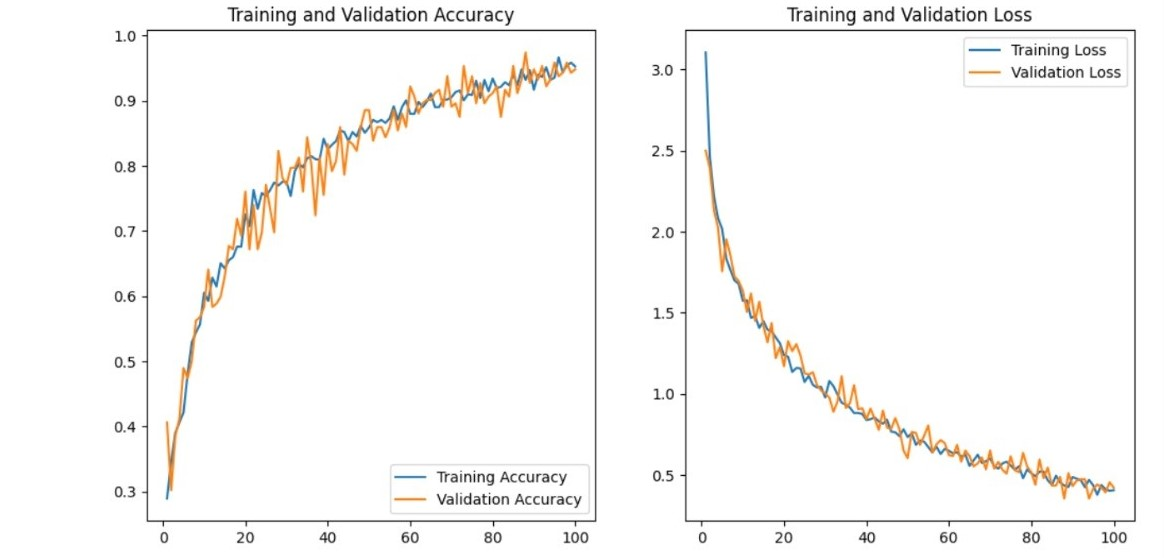
\includegraphics[width=0.6\textwidth]{figs/DenseNet}
	\captionof{figure}{DenseNet121}
	\label{fig:DenseNet}
\end{figure}

\begin{figure}[H]
	\centering
	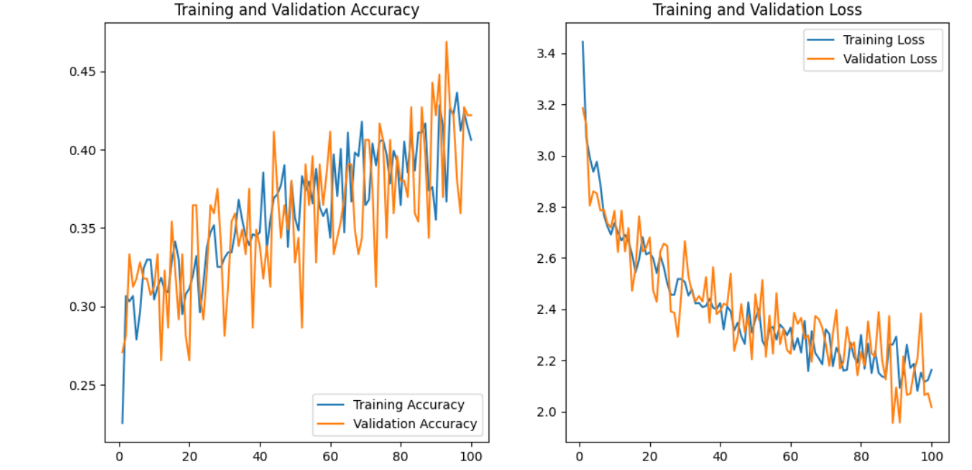
\includegraphics[width=0.6\textwidth]{figs/ResNet}
	\captionof{figure}{ResNet50}
	\label{fig:ResNet}
\end{figure}

\begin{figure}[H]
	\centering
	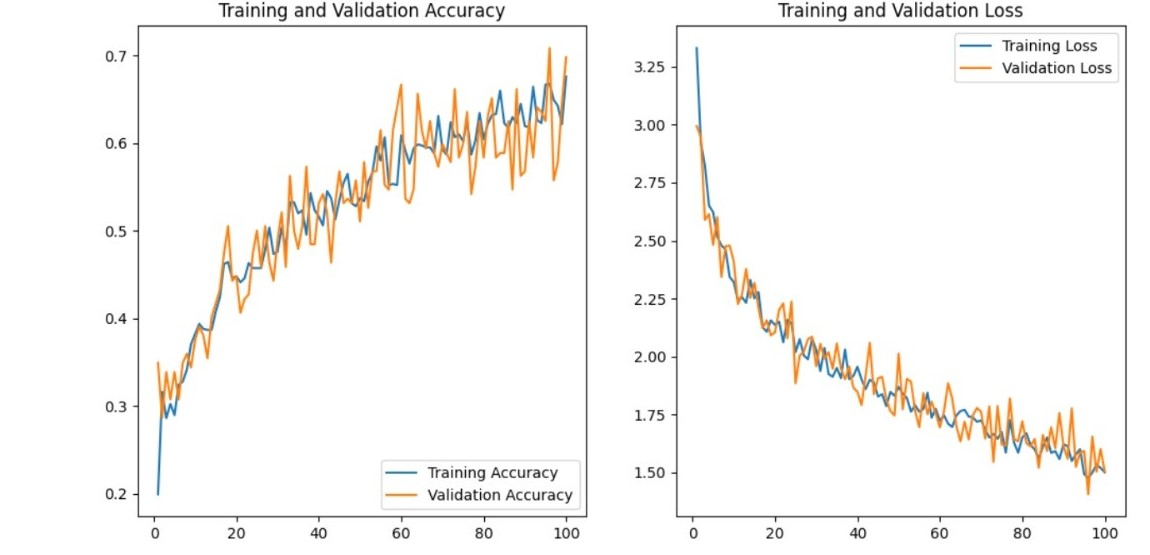
\includegraphics[width=0.6\textwidth]{figs/VGG16}
	\captionof{figure}{VGG16}
	\label{fig:VGG16}
\end{figure}
\vspace{-10pt}
\begin{figure}[H]
	\centering
	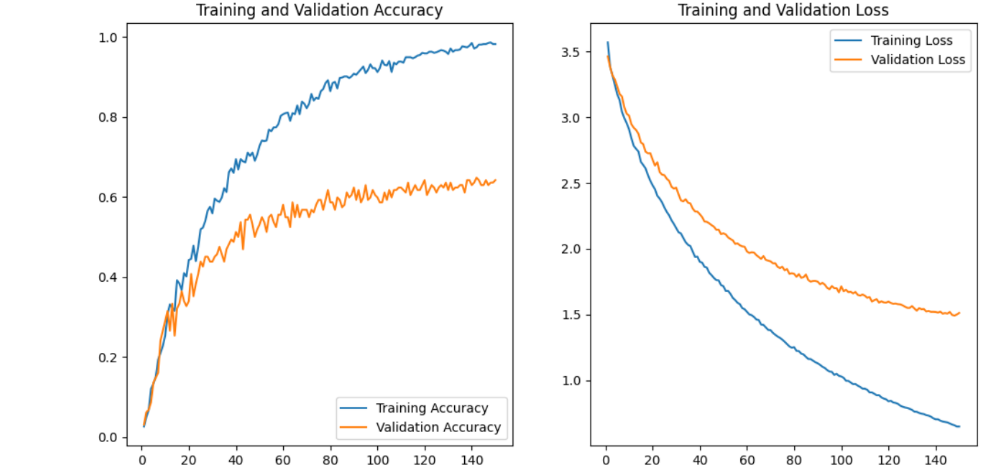
\includegraphics[width=0.6\textwidth]{figs/MobileNet}
	\captionof{figure}{MobileNetv2}
	\label{fig:MobileNet}
\end{figure}


\begin{table}[h!]
	\centering
	\begin{tabular}{|p{5cm}|p{5cm}|}
		\hline
		\textbf{ACCURACY} & \textbf{LOSS} \\ \hline
		
		\multicolumn{2}{|c|}{\textbf{VGG16}} \\ \hline
		Training accuracy: 67.7\% & Training loss: 1.45 \\
		Validation accuracy: 69.8\% & Validation loss: 1.50 \\ \hline
		
		\multicolumn{2}{|c|}{\textbf{DenseNet121}} \\ \hline
		Classification accuracy: 95.2\% & Training loss: 0.42 \\
		Validation accuracy: 94.8\% & Validation loss: 0.42 \\ \hline
		
		\multicolumn{2}{|c|}{\textbf{ResNet50}} \\ \hline
		Training accuracy: 43.3\% & Training loss: 2.09 \\
		Validation accuracy: 42.2\% & Validation loss: 2.01 \\ \hline
		
		\multicolumn{2}{|c|}{\textbf{MobileNetV2}} \\ \hline
		Classification accuracy: 91.5\% & Training loss: 0.98 \\
		Validation accuracy: 59.9\% & Validation loss: 1.71 \\ \hline
		
	\end{tabular}
	\caption{Accuracy and Loss comparison of VGG16, DenseNet121, ResNet50, and MobileNetV2.}
\end{table}

From the results above it can be inferred that DenseNet gives the best results. It's also expected as the model's design naturally benefit tasks where pattern matters.

Hyperparameter fine-tuning emerged as a critical factor influencing the overall performance of the machine learning models. The models, when tuned for optimal learning rates, batch sizes, and regularization parameters, exhibited marked improvements in classification accuracy. It became clear that without rigorous hyperparameter optimization, models tended to either converge too quickly, resulting in suboptimal fits, or fail to converge altogether, as seen during initial training phases. An optimal learning rate, in particular, was pivotal in balancing convergence speed without sacrificing accuracy.

For hyperparameters tuning, base model was frozen and only custom head was trained which is especially useful when we have low data. Also, categorical crossentropy was chosen for classification as it measures difference between predicted class and the true class and encourages model to assign high probability to correct class and low probability to others. Also, since the boxes were normalized in my code MSE (Mean Squared Error) was used as Bounding box prediction is a regression problem. Adam was used as optimizer because it handles small datasets well and a high learning rate of LR = 0-001, helps them learn quickly. Also, in comparison Adam converges faster than plain SGD.

Specific challenges encountered during the training process adversely affected model performance. Issues such as overfitting, poor generalization, feeding the model with incorrect or incomplete data were leading to unstable training, slower convergence and failure to learn meaningful features. Also, images loaded into memory at once created issues with memory and slowing down the program. Also, as the task required 2 outputs, classification + bounding box simple generators such as batch loading struggle to prepare both outputs correctly and efficiently.

Without proper data generator I ended up with mismatched data shape and incorrect labels. 

\begin{figure}[H]
	\centering
	\fbox{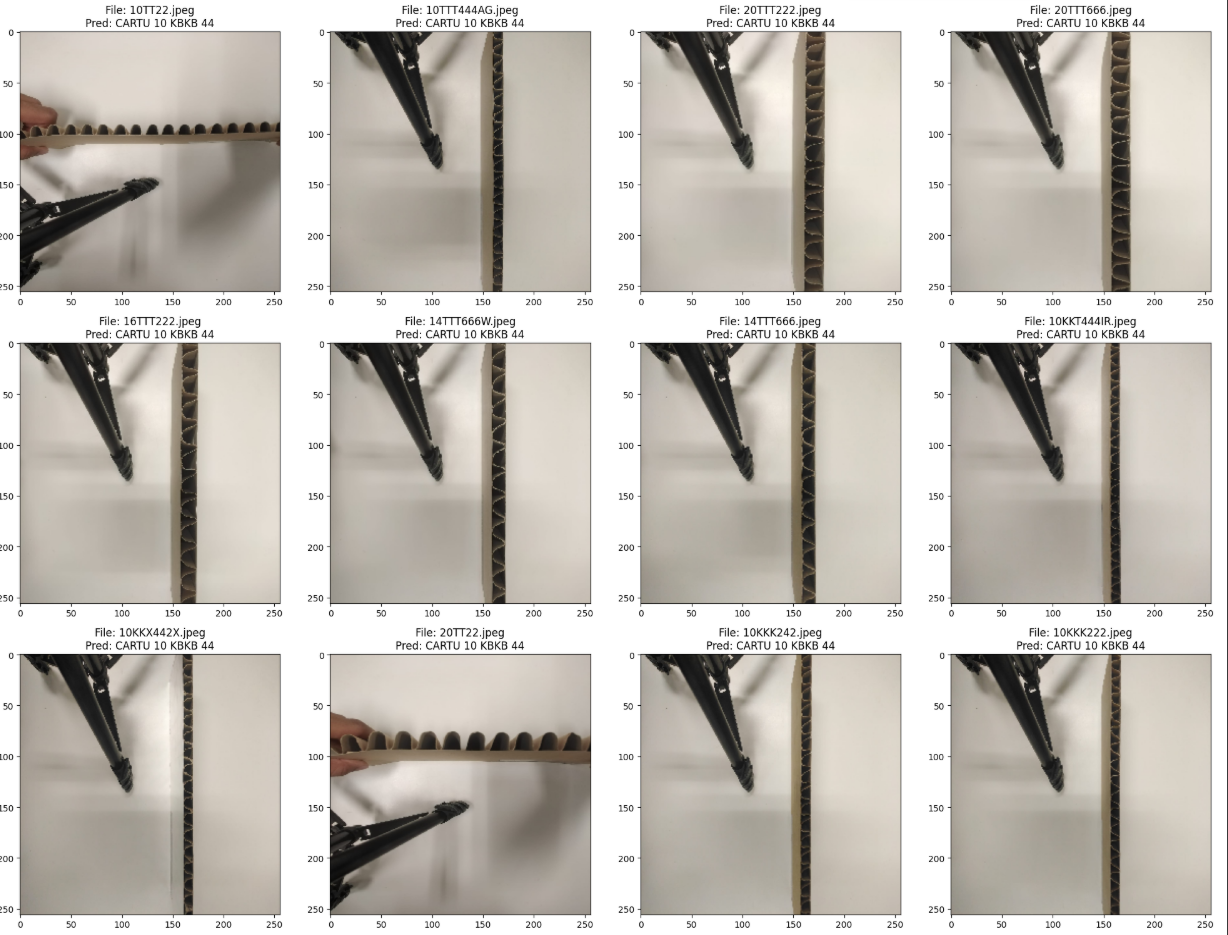
\includegraphics[width=0.6\textwidth]{figs/Data}}
	\captionof{figure}{Image Detection without Proper Data Generator}
	\label{fig:Data}
\end{figure}


To overcome this, custom data generator was made. This allowed for better resilience against the model memorizing rather than learning from the training data.  It helped with dynamic shuffling and also shuffles data every epoch, improving generalization and helping against overfitting and biased training. It also ensures correct label alignment and skips missing or invalid samples. Most importantly, it helped with memory management and helped with better load times, particularly beneficial with tasks where resources are limited.

The influence of different data augmentation techniques on the robustness and accuracy of the models was substantial. Data augmentations are although necessary to implement in many cases, in cases which I was working on showed very minute differences between cardboards. The introduction of transformations like rotation, flipping, and intensity adjustments can vastly increase the diversity of training images available to models, thus improving their ability to generalize. Earlier evaluation of performance metrics post-augmentation indicated decrement in classification accuracy, leading to application of fewer and fewer augmentations.

The relationship between the quality and volume of training data and final model performance was another significant consideration. Initial findings suggested that models trained on larger, well-distributed datasets yielded better generalization to unseen data. However, fluctuations in dataset quality stemming from inconsistency in image resolution and lighting conditions significantly affected model reliability and such images had to be deleted. However, it can be established that moderately high accuracy can be achieved with less data as well for cases where not enough data is present. Also, this saves from needing expensive model training equipment and devices, especially in case of edge devices where replication of the results to broader fields feels challenging due to the costs.

Valuating model predictions against a diverse set of testing images unveiled insights regarding specific design features of cardboard flutes, enhancing understanding regarding which characteristics held decisive weight in classification decisions. Instances of misclassification often correlated with similarities between flute designs that were not sufficiently addressed during the training phase, leading to implications for future data collection strategies that promise a more diverse selection of flute representations. 

The incorporation of instance segmentation techniques into the evaluation phase allowed further exploration into the recognition accuracy for cardboard flute classification. By enhancing the extraction of boundaries and features typically obscured in traditional object detection, models benefitted from improved localization and subsequently, a refined classification approach. This intersection of methodologies showcased the importance of integrating multiple techniques to bolster overall model efficacy.

Environmental factors, including variable lighting and background conditions during image capture, played a defining role in the accuracy of model predictions post-training. The diverse operational contexts that cardboard flutes may appear in highlighted the need for extensive preprocessing and augmentation strategies that adequately prepare data for robust training opportunities. As models transitioned from controlled environments to unpredictable real-world conditions, the breadth of variation became a critical factor in their operational success.

In summary, the analysis of training results illustrated the myriad factors influencing the efficacy of machine learning models in classifying cardboard flutes. Through methodologies focused on optimizing architectures, tuning hyperparameters, addressing training challenges, and harnessing the power of data augmentation, this highlights the complexity inherent in achieving significant advances in classification accuracy. As ongoing research continues to refine these practices, it becomes evident that nuances within training methodologies will remain pivotal to the enhancement of model performance in this domain.

%--------------------------------------------------------------------------
\section{Comparison with Existing Methods}
%-------------------------------------------------------------------

This section tells about the advantages gained from the techniques we used. Traditional algorithms, while effective in their time, often struggle with the increased complexity and dimensionality of image classification tasks, especially those involving intricate objects like cardboard flutes

The integration of instance segmentation techniques is another area where modern approaches surpass previous methods. Traditional classifiers often analyze whole images without acknowledging the importance of object boundaries, leading to potential misclassifications. In contrast, instance segmentation models like those enabled by YOLOv8 can accurately delineate the contours of objects, thereby enhancing classification accuracy. 

Real-time interaction with a web interface are pivotal components that elevate the performance of machine learning models compared to static testing environments encountered in traditional approaches. Traditional classifiers often rely heavily on pre-set baseline conditions and limited interactions, which do not foster adaptive learning. In contrast, a real-time, user-driven interface allows machine learning models to evolve through continuous feedback loops. When users upload images of cardboard flutes, their insights can provide actionable data that informs model adjustments, contributing to a more robust classification model. This interactivity leverages the fine-tuning capabilities of contemporary systems, allowing for a dynamic exchange of knowledge between technology and factory processes.

A crucial element in understanding the comparative performance of machine learning models lies in the architecture differences, particularly between deep learning. The deep learning architectures not only excel in detecting finer patterns but also adaptively improve as they process more data. This aspect is particularly salient when training models on diverse datasets, which significantly impacts their generalization capabilities. The traditional methods tend to suffer when faced with variability in data quality, often requiring extensive feature engineering and manual tuning. In contrast, the automated feature extraction potential of convolutional neural networks (CNNs) leads to performance improvements across varied representations of cardboard flutes.

However, deploying models with advanced deep learning techniques presents distinct challenges that differ from those encountered with traditional methods. The computational resources required for training, the need for large, well-balanced datasets, and the complexity of tuning hyperparameters present both a barrier and an impetus for advancement in machine learning. These requirements pose difficulties, especially when resources are constrained. In contrast, traditional methods may offer lower computational demands but at the cost of robustness and adaptability.

Ultimately, the comparison between existing methods and the proposed machine learning techniques within this study underscores the evolution of pattern recognition approaches in the domain of cardboard flutes. The innovations presented by machine learning algorithms significantly advance the capability of classification systems, particularly as they adapt to the unique challenges posed by similarities in patterns of cardboard flutes. Importantly, recognizing and addressing the limitations of both traditional and modern methodologies will guide future developments in this exciting area of research.

In our experiments, the integration of DenseNet for feature learning and YOLOv8 for instance segmentation demonstrated clear benefits compared to alternative architectures. DenseNet consistently captured fine-grained structural details in the cardboard patterns, which translated into higher classification consistency even under challenging conditions such as varying distances and lighting. The dense connectivity proved particularly effective in preserving subtle textural differences, reducing the risk of feature loss across layers.

When combined with YOLOv8-Seg for detection and mask generation, the approach provided both accuracy and efficiency. The model was able to not only localize each cardboard piece but also generate precise segmentation masks, effectively separating overlapping instances.

Overall, the DenseNet + YOLOv8 pipeline outperformed traditional classification-only or detection-only approaches by ensuring both robust feature representation and accurate instance-level segmentation. This dual advantage allowed the system to generalize better across diverse test conditions and offered practical reliability for downstream applications where both speed and precision are required.


%--------------------------------------------------------------------------
\section{Real-World Applications of the Model}
%-------------------------------------------------------------------
This section examines the practical implications of machine learning techniques for the classification of cardboard flutes, also focusing on instance segmentation and user engagement through a web interface. The application of advanced optical recognition methodologies within such domains not only enhances the classification precision but also opens avenues for increasing user creativity and accessibility. The exploration of real-world implementations illustrates how machine learning can be democratized to increase participation from all the industrial sectors, particularly for those with limited access to traditional training or recognition systems.

The implementation of instance segmentation techniques stands out as a crucial advancement in accurately classifying cardboard flutes under varying environmental conditions. Models trained to recognize the distinct features of these can rely on a well-prepared dataset that encompasses numerous representations of the flutes in different settings. This vital capability ensures that machine learning models become increasingly equipped to handle the intrinsic variations in features and presentations which characterize items like cardboard flutes.

In developing a user-focused web interface for real-time image upload and analysis, several features and functionalities emerge as priorities. A seamless experience necessitates employing intuitive designs that allow users of varying technical capabilities to engage with the system effortlessly. Implementing drag-and-drop functionalities empower users to submit their images quickly.

The successful collaboration between researchers, technology experts, and professionals can yield enriched training datasets that capture a broad spectrum of objects. Such partnerships may bring additional perspectives on what constitutes essential features within such designs, challenging existing paradigms and fostering the creation of innovative models that are responsive and adaptable to diverse fields. As machine learning applications evolve, their implementations can not only be used for a single-use case and the same models can be applied at various places. For instance, research on cardboard flutes can be very helpful for medical images as well where we can have rare conditions, small differences and limited availability of data.

In conclusion, the real-world applications of machine learning for classifying cardboard flutes serve multiple purposes by improving accuracy, enhancing user engagement, and promoting ethical standards in technology deployment. The combination of instance segmentation techniques, user interactions through web interfaces, and collaborative efforts between technology and the different sectors offer a comprehensive model for bridging modern technology with the traditional industries. This section highlights the exciting potential these methodologies uphold, paving the way for future advancements.


%--------------------------------------------------------------------------
\section{Future Directions for Research}
%-------------------------------------------------------------------
In the rapidly evolving field of pattern recognition through machine learning, the classification of cardboard flutes presents intriguing opportunities for future research. Identifying the implications of improving data quality and diversity is crucial for enhancing the accuracy of deep learning models specific to cardboard flute classification. With increasing evidence that the richness of data can enhance model performance, future studies should focus on identifying optimal strategies for data collection, such as leveraging community contributions to create diverse datasets that represent various flute designs, materials, and lighting conditions. It will be important to investigate how these factors influence not only accuracy but also the robustness of the models against overfitting in real-world applications.

An additional avenue for exploration lies in integrating community engagement and user feedback into machine learning systems. By establishing platforms for users to interact with models and provide insight regarding classification results, researchers can facilitate adaptive learning mechanisms that reflect actual usage scenarios. This participatory approach can lead to customized model improvements, enhancing adaptability and accuracy in response to unconventional flute designs or user preferences. Insights from diverse user experiences can bridge theoretical advancements with practical functionality, positioning future research at the intersection of machine learning and user engagement.

Examining the influence of varied lighting conditions emerges as another valuable direction for systematic research within image recognition systems. The performance of deep learning models suffers substantially when subjected to inconsistent lighting, which can obscure or distort object recognition. Future studies should rigorously investigate preprocessing techniques, such as normalization and enhancement algorithms, that can alleviate the challenges posed by dynamic lighting conditions. Researchers may also explore the effectiveness of data augmentation methods that mimic these variations during training, thus equipping models with the resilience needed to operate under real-world circumstances.

Interdisciplinary collaborations will be essential for advancing machine learning applications in the classification of cardboards. The integration of insights can foster innovative approaches that consider these nuances in a more detailed manner during algorithm development. Collaborations could lead to the creation of custom models that cater specifically to the unique attributes of cardboard flutes, enhancing predictive accuracy. By bridging technological expertise with industry, future research can create holistic solutions for complex classification challenges.

Refining instance segmentation techniques can further advance the detection of intricate patterns. By employing enhanced algorithms tailored for complex designs, future research could unlock new capabilities in segmentation that improve model accuracy for visually rich tasks such as cardboard flute classification. This refinement may encompass advancements in training methodologies, enabling models to better recognize subtle variations in design and material.

Moreover, real-time feedback mechanisms must be integrated within the system to inform users about the status of their uploads and the outcomes of the classification process. Such interactive elements can significantly enhance user satisfaction, thereby cultivating a supportive environment that encourages creativity and exploration.

Integrating user feedback into the model training process presents another innovative approach to enhancing the system's robustness and classification accuracy. By allowing users to provide insights regarding the effectiveness of the classifications and report inaccuracies, the models can undergo iterative refinement. Users often have an intimate understanding of the objects they submit, and their input can elucidate aspects that may not have been fully captured during the initial training phase. The influence of such an interactive feedback mechanism underscores the importance of fostering a collaborative atmosphere between technology and industry.

Exploring the role of transfer learning holds promise for enhancing model performance in niche classification tasks, especially with limited datasets. By utilizing pre-trained models on large benchmark datasets, researchers can adapt them for specialized classification of cardboard flutes, effectively reducing training time and promoting higher classification accuracy. Understanding the nuances of transfer learning as it relates to such domains presents an exciting area for further investigation, revealing how pre-existing knowledge can be effectively harnessed for more intricate tasks.

As scalability becomes an increasing concern for machine learning models, future research should focus on optimizing systems to handle variable volumes of user-generated images without sacrificing classification accuracy. Investigating modular architectures that facilitate efficient handling of substantial data influxes can help overcome the computational challenges associated with large-scale applications.

Best practices in deploying machine learning systems across various platforms also warrant attention to ensure consistent and reliable performance for users. Future studies should examine how semi-automated workflows can adapt to different environments, allowing for seamless integration of models into diverse applications while maintaining high standards of classification reliability.

Additionally, maintaining data privacy and security in web-based machine learning applications directed towards the manufacturing sector is also pivotal. Users must be assured that their creative contributions are safeguarded, and their privacy is respected. Implementing robust data protection measures while transparently communicating policies regarding user data is crucial in fostering trust and encouraging wider participation in machine learning frameworks.

Lastly, incorporating ongoing technical maintenance and system monitoring into machine learning applications is vital to ensure sustained efficacy in pattern recognition. Future research should develop frameworks that monitor systems continuously, allowing for timely updates and adjustments based on emerging trends in user behavior and operational metrics. This proactive approach will guarantee that machine learning applications continue to meet the evolving needs of the community while ensuring robust performance in pattern recognition tasks. 

By charting these future directions for research, scholars and practitioners alike can contribute to the continuing evolution of machine learning technologies, fostering innovation in the classification of cardboard flutes and other related endeavors.
